%\documentclass[12pt,a4paper]{article}
%
%\usepackage{amsmath, amssymb}
%\usepackage[utf8]{inputenc}
%\usepackage[english]{babel}
%\usepackage{graphicx}
%\usepackage[margin=0.5in]{geometry}
%\usepackage{float}
%
%\graphicspath{{fig/}}


%\begin{document}

%\section{Writing Controller Code}
\subsection*{Level 1}
The code equivalent to the Simulink blocks gave similar results which
can be seen in Figure \ref{fig:task2_traj} and
Figure~\ref{fig:task2_pos}. A sampling time of 10 ms was used for the
code. Different sampling times were tested and it was noticed that
when using a higher sampling time the impact on the trajectory planner
increased. When a higher sampling time was used the change of
acceleration is missed by a few milliseconds and is therefore impacting the
velocity and position. This gives the difference in the position of the
motor which is seen in Figure \ref{fig:task2_pos}.
\begin{figure}[H]
	\begin{center}
	
		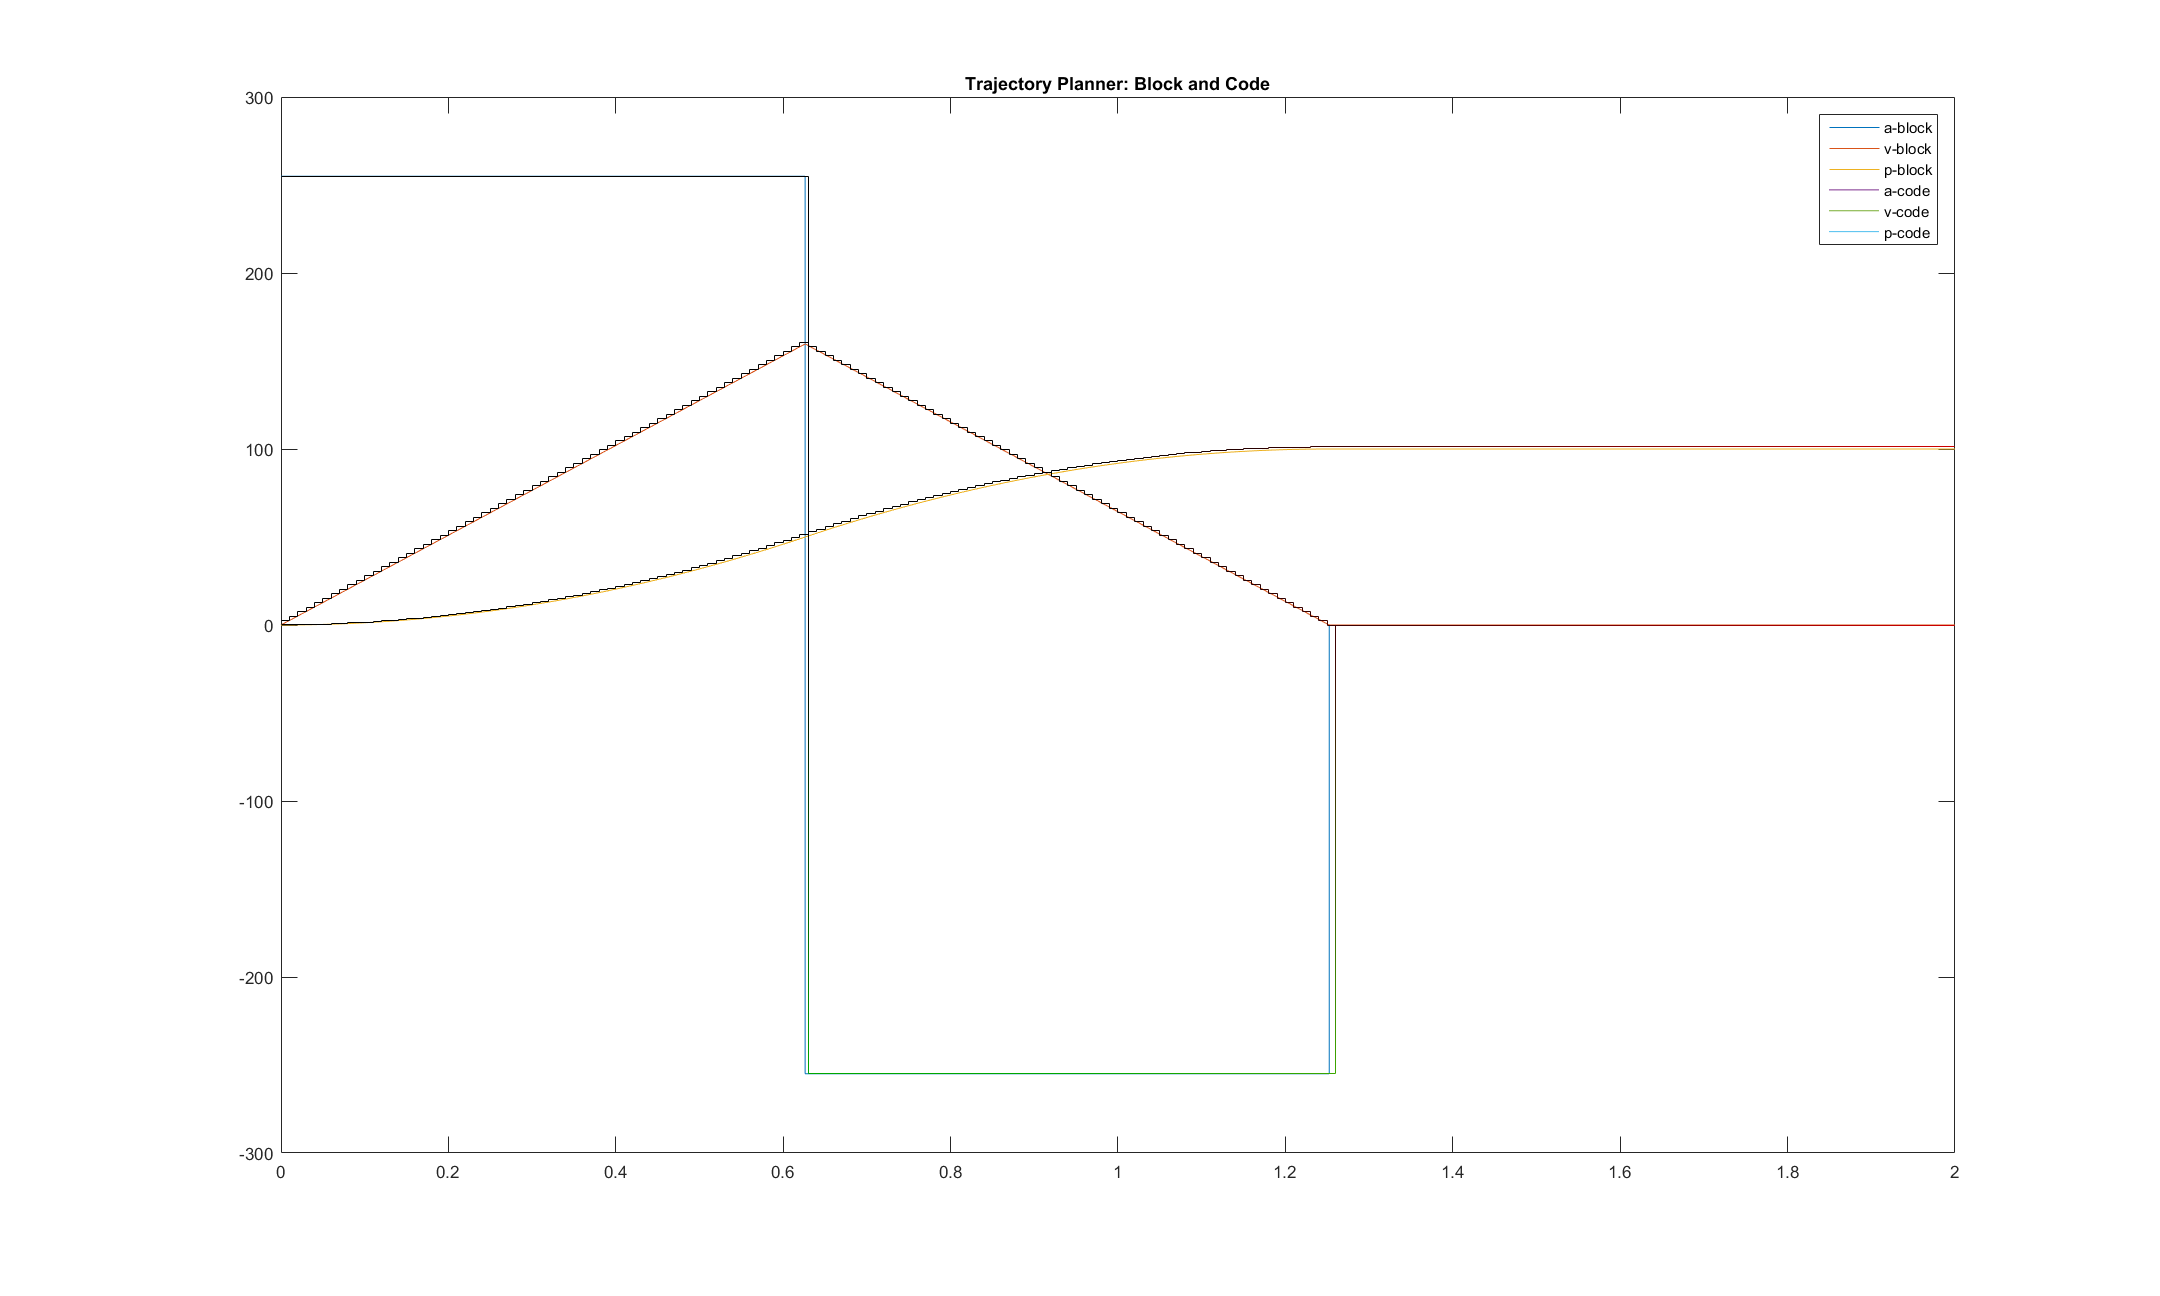
\includegraphics[width=0.45\linewidth]{task2_traj.png}
		\caption{Trajectory planner signal comparison}
		\label{fig:task2_traj}
	\end{center}
\end{figure}
\begin{figure}[H]
	\begin{center}
	
		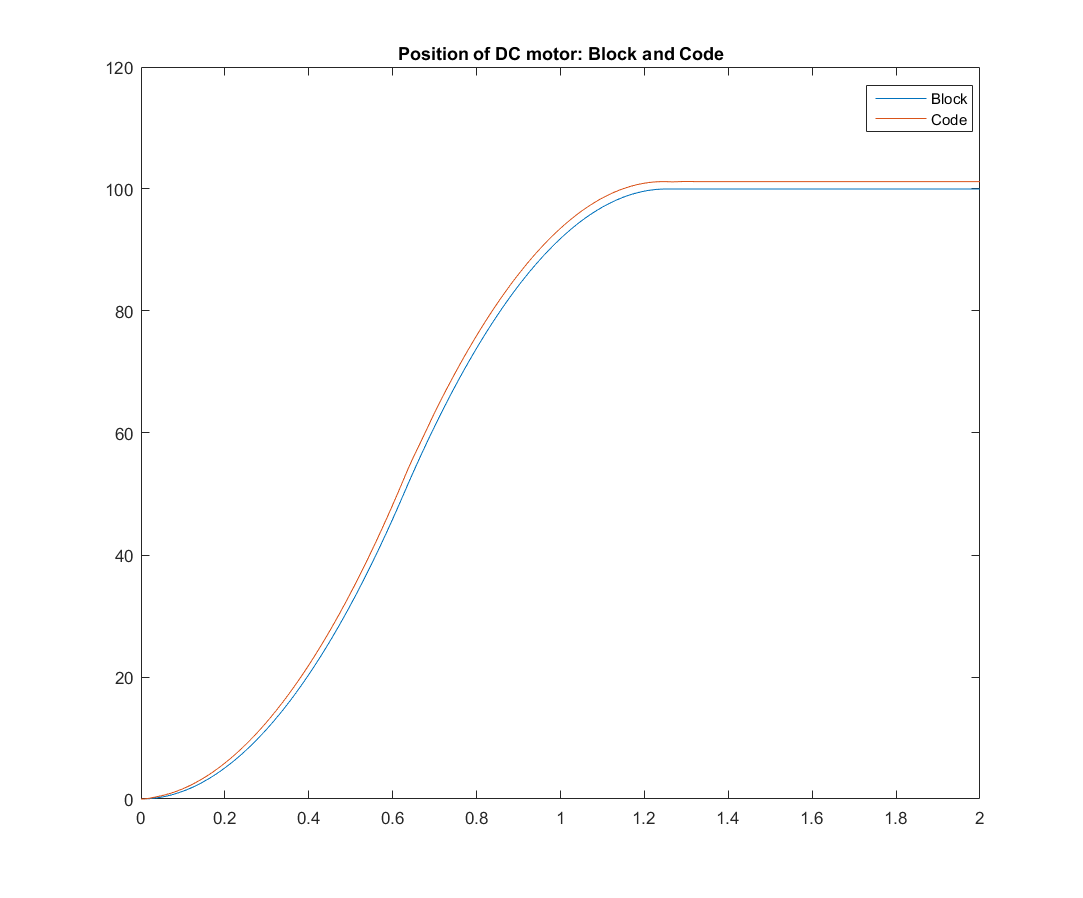
\includegraphics[width=0.45\linewidth]{task2_position.png}
		\caption{Motor position comparison}
		\label{fig:task2_pos}
	\end{center}
\end{figure}

A close-up of the sampling time problem is shown in Figure
\ref{fig:task2_closeup}. When the velocity increases it the code signal
follows the curve perfectly but when there is a change in acceleration
the velocity code signal gets "out-of-sync".

\begin{figure}[H]
	\begin{center}
	
		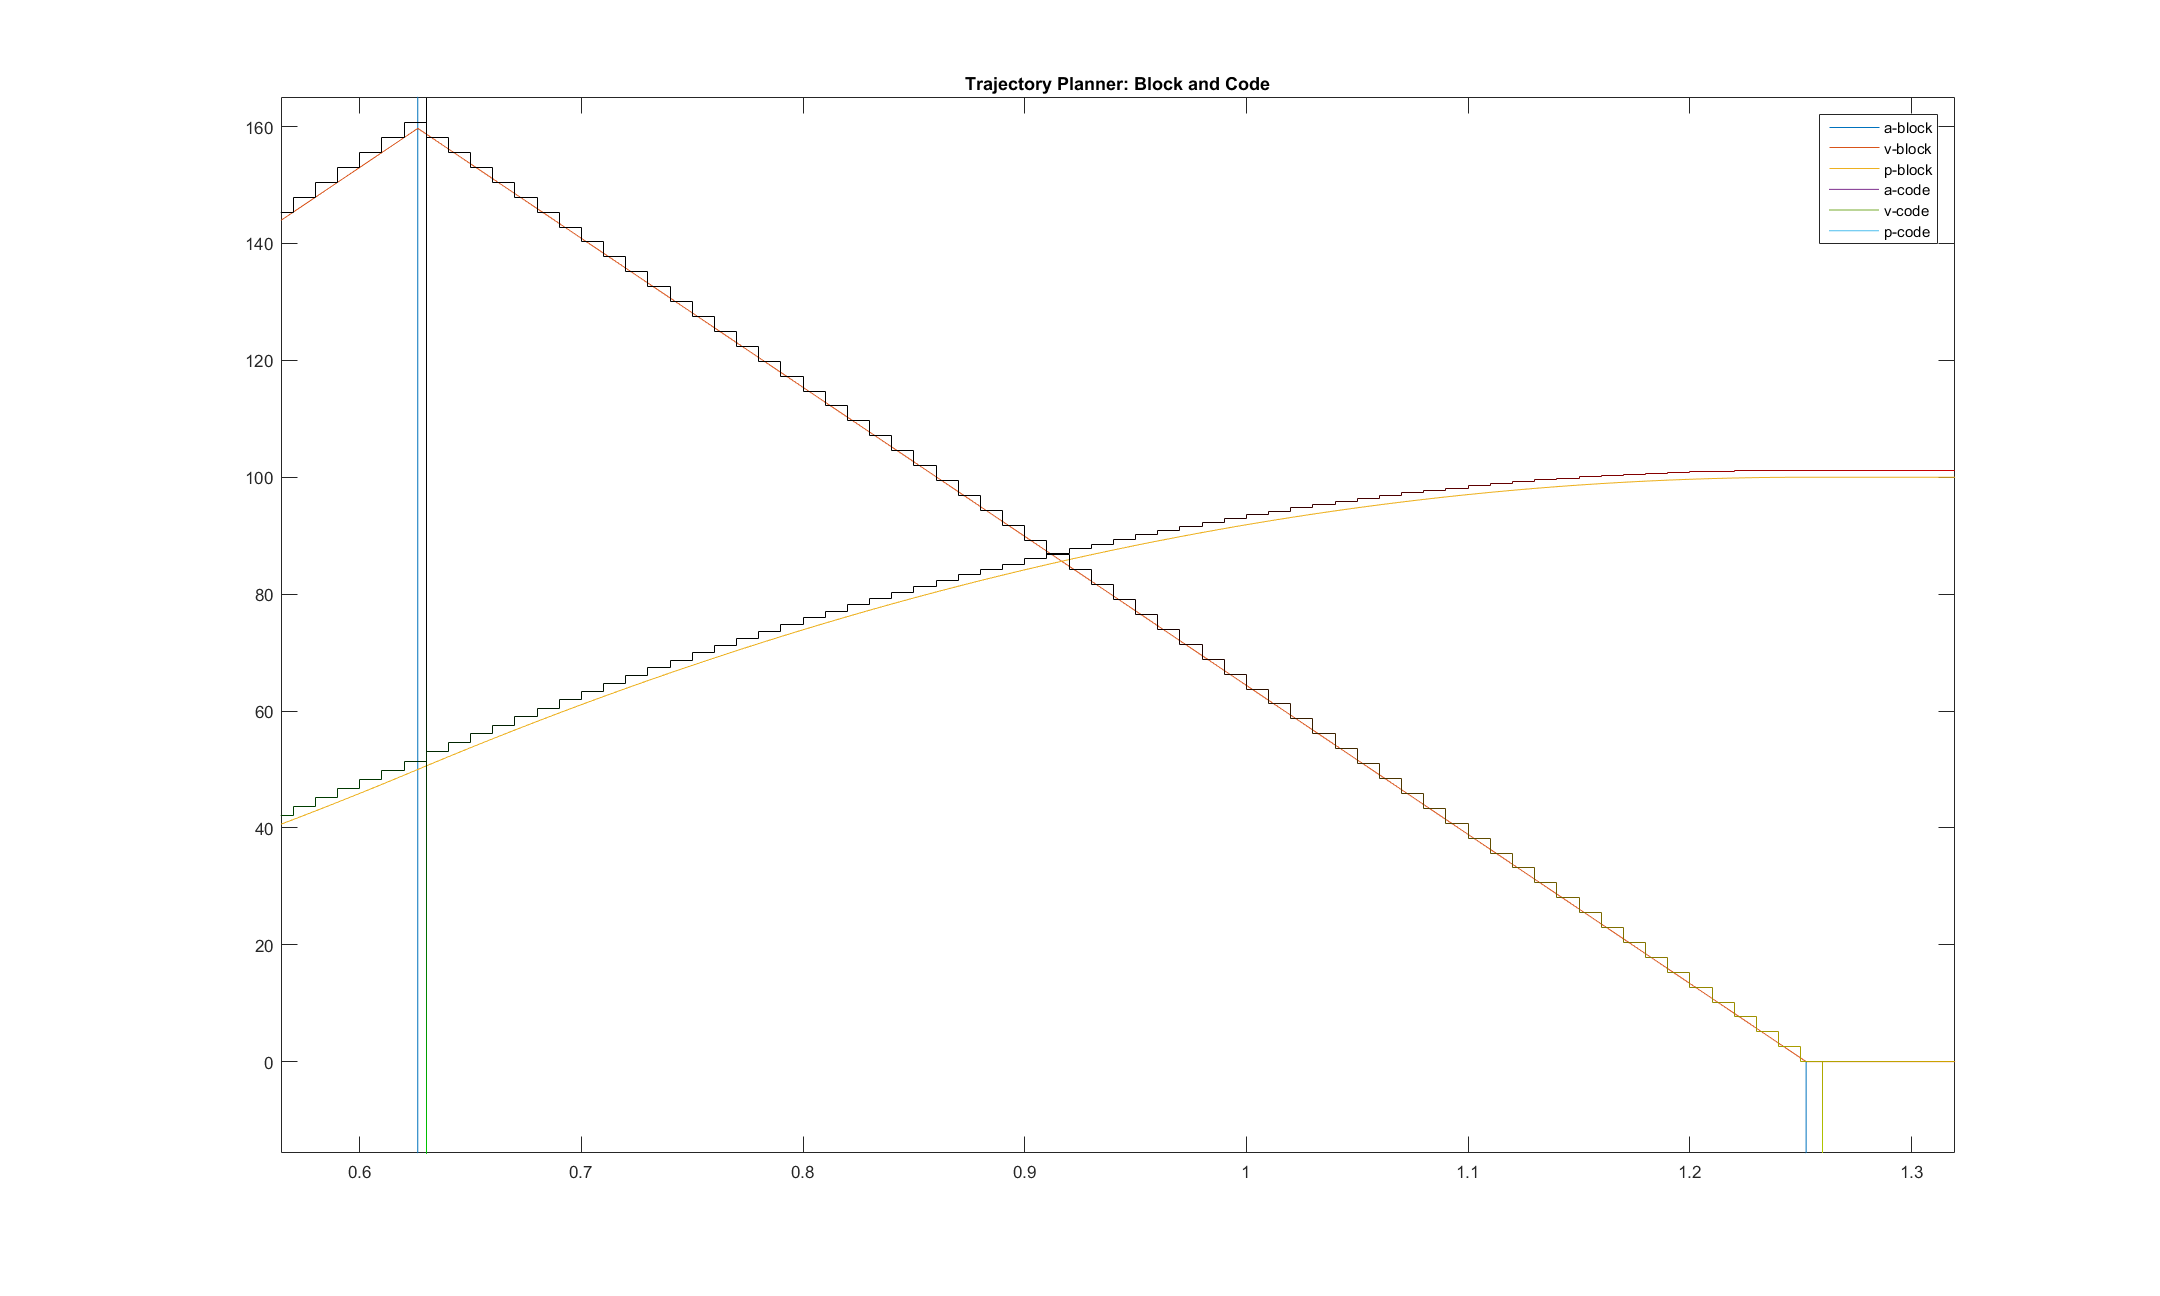
\includegraphics[width=0.45\linewidth]{task2_closeup.png}
		\caption{Close-up of trajectory planner signal}
		\label{fig:task2_closeup}
	\end{center}
\end{figure}


\subsection*{Level 2}
Some modifications to the code had to be made to make it work in dSPACE
but the same code is used for the plot in Figure
\ref{fig:task2_traj_l2}. The performance of the trajectory planner in
dSPACE worked excellent. It behaved almost exactly like in Simulink on
the DC-motor model. 
\begin{figure}[H]
	\begin{center}
	
		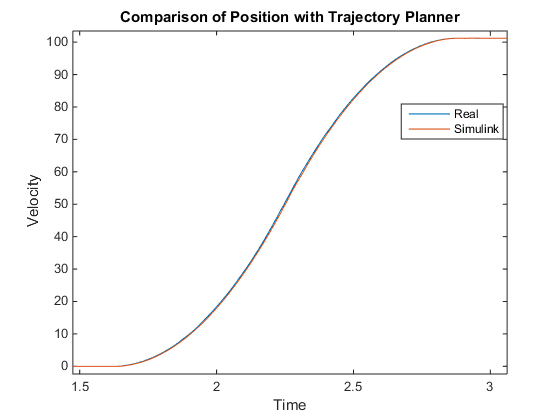
\includegraphics[width=0.45\linewidth]{task2_traj_l2.png}
		\caption{Comparison on the performance of the trajectory planner}
		\label{fig:task2_traj_l2}
	\end{center}
\end{figure}
The code for the embedded controller can be found in Listing 1.
\lstdefinestyle{customc}{
breaklines=true,
  frame=L,
  xleftmargin=\parindent,
  language=Matlab,
  showstringspaces=false,
  basicstyle=\footnotesize\ttfamily,
  keywordstyle=\bfseries\color{green!40!black},
  commentstyle=\itshape\color{purple!40!black},
  identifierstyle=\color{blue},
  stringstyle=\color{orange},
}
\lstinputlisting[caption=Embedded Matlab Code, style=customc]{ControllerC.m}
%\end{document}
